\documentclass[a4paper,10pt]{article}
\usepackage[utf8]{inputenc}
\usepackage{hyperref}
\usepackage[
    type={CC},
    modifier={by-sa},
    version={4.0},
]{doclicense}

%opening
\title{Pay-to-TagAddress (P2TA): Tagging blockchain transactions for efficient queryability}
\author{Hans Robeers\\ \texttt{hrobeers@protonmail.com}\\ \url{https://twitter.com/hrobeers}}

\begin{document}

\maketitle

\begin{abstract}
Multiple applications are using existing blockchains as a communication network.
Most of these implementations are scanning to blockchain for transactions matching their own format.
However, this requires a full blockchain node and processing a large blockchain to find application specific transactions can become expensive to execute.
This paper proposes a tagging mechanism, Pay-to-TagAddress (P2TA), that allows efficient lookup of application specific transactions based on the addition of transaction outputs to deterministic tagged addresses. P2TA also allows thin clients to find application specific messages using standard functions exposed by the widely available blockchain explorers.
\end{abstract}

\doclicenseThis

\section{Introduction}
Blockchains, as first introduced by the Bitcoin~\cite{Nak08} network, are used increasingly by third-party applications.
Examples of third-party usage includes Colored Coins~\cite{Ros12}, PeerMessage~\cite{Emeth}, PeerAssets~\cite{Pchem} and multiple others.
These applications typically publish there own specific messages in the form of OP\_RETURN transaction outputs on a third-party blockchain.

Scanning an entire blockchain for messages of a specific form becomes increasingly expensive while the blockchain grows.
Applications like PeerMessage~\cite{Emeth} only rely on real-time transactions being relayed by the network and therefore do not suffer from blockchain growth.
However, applications like PeerAssets~\cite{Pchem} need know an entire history of asset specific transactions to be able to validate asset ownership.
Therefore these type of applications would greatly benefit from a system that allows efficient querying of transactions holding a specific tag.

Blockchain growth also increases disk and memory usage of the full nodes needed to parse the blockchain for application specific messages. For lightweight applications, downloading the entire blockchain might become infeasible. A query mechanism to find these messages using standard lookup functions, would allow these third-party applications to be implemented as thin clients interfacing with standard blockchain explorers like blockr.io \cite{Blockr}.

\section{Blockchain queryability}
Blockchain clients are designed to efficiently query for transactions, blocks and addresses by their ids.
Therefore the client can be approached as if it's storing the blockchain indexed on transactions, blocks and addresses.
Querying for non-indexed data on the blockchain can be considered inefficient and to be avoided and might even be infeasible using a thin client.
For efficient queryability of application specific transactions on the blockchain, a tagging mechanism based on the indexed properties can be used.

\section{Deterministic tagged address}
\label{sec:taggedaddress}
Blockchain addresses are typically created by hashing the public key of a public/private key pair.
To generate secure addresses it is recommended to use a strong random number as a private key.
However, as long as little or no funds are transferred to an address, there is no need for the address to be secure to theft.
Therefore private keys obtained by hashing a publicly known string can generate what we call a deterministic tagged address.

As an example, the command below demonstrates how a tagged address for tag ``my tag'' on the bitcoin network can be created using bitcoin-tool~\cite{Matja}, that can be used for different blockchain networks.

\begin{small}\begin{verbatim}
$ bitcoin-tool --input-file <(echo "my tag" | openssl sha256 -binary) \
               --input-type private-key \
               --input-format raw \
               --network bitcoin \
               --output-format base58check \
               --output-type address \
               --public-key-compression compressed
194aYsKYk7nF8Lf7Dak4vQaDg85wqPDy1g
\end{verbatim}\end{small}

\section{Tagging transactions}
To tag a transaction, a Pay-to-PubkeyHash output to a tagged address is added to the transaction's outputs.
For the output to be valid, it's value may need to be non-zero depending on the blockchain used.
Although this transaction output is indistinguishable from a standard Pay-to-PubkeyHash output, we refer to these outputs as Pay-to-TagAddress or P2TA in short.

If we define the function \verb|address_for_tag(tag)| as the procedure described in section~\ref{sec:taggedaddress}, the following bitcoin command creates a tagged transaction with tag ``my tag''.

\begin{small}\begin{verbatim}
createrawtransaction [{ "txid": txid, "vout": n }]
    {
      address: amount,
      change_address: change_amount,
      address_for_tag("my tag"): minimum_amount
    }
\end{verbatim}\end{small}

Note that most networks implement dust spamming counter measures which are triggered the by low output amount of the tag output.
Make sure to check with the involved communities if these transactions are acceptable on their network.


\section{Querying tagged transactions}
Most blockchain clients can efficiently query addresses and their linked transactions by their id.
Efficiently finding transactions tagged by a known tag is done as follows:
\begin{itemize}
 \item Generate the tagged address as described in section~\ref{sec:taggedaddress}.
 \item Query the generated address.
 \item The tagged transactions are the incoming transactions on this address.
\end{itemize}


\section{Tag salting}
Tags are usually human readable and human generated rather than randomly generated.
There is a high probability for tags not to be unique.
Therefore, applications using P2TA should be able to cope with unrelated transactions coming in on the tagged address, and lower the client's performance.
A reasonable technique to lower the risk on tag collisions, is adding a publicly known salt to the tag.
This salt might be hard coded in the client application or be randomly generated and broadcast to the public.
It should be noted that salting cannot mitigate intentional ``tag spamming'', but it mitigates unintentional collisions.


\section{Tag spamming}
P2TA applications can be attacked by spamming their tag addresses.
Tag spamming can reduce the applications performance significantly by increasing the amount of required transaction lookups.
In extreme cases it could even result in a full denial of service (DoS attack).
This section proposes counter measures to ``tag spamming''.

\subsection{Sent address black-listing}
While parsing the tagged transactions, addresses sending many application unrelated messages to the tagged address can be blacklisted.
The P2TA application can then ignore all transactions originating from the blacklisted addresses.
This counter measure is quite naive, as spammers can easily use a different address for every spam message.
It might also happen that legitimate addresses get blacklisted therefore compromise the proper functioning of the application.

\subsection{Proof-of-Burn}
An application can require the P2TA output to burn a specific amount,
which would make it costly for attackers to execute a DoS attack.
Spam transactions would still show up in the incoming transaction lookup for the tagged address,
but the client can ignore all transactions below the threshold amount.
Proof-of-Burn requires the P2TA output to be unspendable, meaning that the private key should not be recoverable from the tag and salt.
Therefore a different address generation procedure is required for a Proof-of-Burn protected implementation.
Instead of generating the private key, we propose to generate the public key as the hash of the tag + salt.

Using bitcoin-tool on the bitcoin network this looks as follows:

\begin{small}\begin{verbatim}
$ bitcoin-tool --input-file <(echo "tag and salt" | openssl sha256 -binary) \
               --input-type public-key-sha \
               --input-format raw \
               --network bitcoin \
               --output-format base58check \
               --output-type address \
               --public-key-compression compressed
12w3JJ84RXmJUZTgafJJ91vvLg8oU5djUG
\end{verbatim}\end{small}

Note that the Peercoin~\cite{King12} implements a Proof-of-Burn mechanism by requiring a transaction fee of 0.01PPC per kb transaction size.
However, this fee might still be too low to effectively prevent ``tag spamming''.

\subsection{Spam filtered blockchain explorer}
A standard blockchain explorer API can return all transactions on a specific address.
This functionality is used to discover all transactions related to a specific tag.
Applications can decide to expose a similar web service method that only returns valid application specific transactions.
This centralises spam filtering and therefore increases the thin client's performance.
It should be noted that this introduces a single point of failure.
Therefore it is recommended to implement fallback service calls using third-party unfiltered blockchain explorers.

\subsection{Hierarchical deterministic wallets}
BIP32~\cite{Wui12} proposes a mechanism to generate a fully deterministic tree of private or public keys based on a single seed.
The tag and salt can be used as the seed to generate such a tree.
Applications that model their messages as a chain of transactions can use such a tree to map it's messages on.
Finding all transactions with a single tag, becomes considerably more expensive than for a single tag address as it requires an extra address lookup for every application message.
However, since every message has a unique tag address, attacking the entire application by ``tag spamming'' becomes practically infeasible.


\section{Use case: PeerAssets}
This section proposes a performance improvement to the PeerAssets~\cite{Pchem} paper as a use case.
Contrary to the Peershare~\cite{Lee13} project that creates it's own blockchain, the PeerAssets paper proposes a way to register, distribute and trade assets on the Peercoin~\cite{King12} blockchain.
A naive implementation of P2TA could take the form of adding a simple ``PeerAssets'' tag to every PeerAssets specific transaction, which would allow a thin client to parse only the application specific transactions.
However, a slightly more advanced tagging mechanism is proposed in this section.

\subsection{Deck spawning}
The process to register a new asset on the blockchain is referred to as ``deck spawning''.
A deck is spawned by publishing a message that claims ownership over a specific asset. From that point on, only the spawning address is allowed to issue tokens of that asset.
Therefore, an efficient lookup mechanism to check if a specific asset already exists without the need to parse all blockchain transactions, improves the client's performance considerably.
For deck spawning lookup, one P2TA output for tag \verb|"PeerAssets/deck spawning"+salt|, is added to the transaction.
The resulting transaction outputs for a deck spawning transaction look as follows:

\begin{scriptsize}\begin{verbatim}
OP_RETURN <data>
OP_DUP OP_HASH160 <change_address_pk_hash> OP_EQUALVERIFY OP_CHECKSIG
OP_DUP OP_HASH160 <pk_hash_for_tag("PeerAssets/deck spawning"+salt)> OP_EQUALVERIFY OP_CHECKSIG
\end{verbatim}\end{scriptsize}

Figure \ref{fig:txn_relations} illustrates the different transaction properties needed to create a ``Deck spawn txn''.
The create\_txn\_id is it's default transaction id being the hash of the transaction.
This idea will be used to link asset transactions to their deck spawning transaction.

\begin{figure}[h]
 \centering
 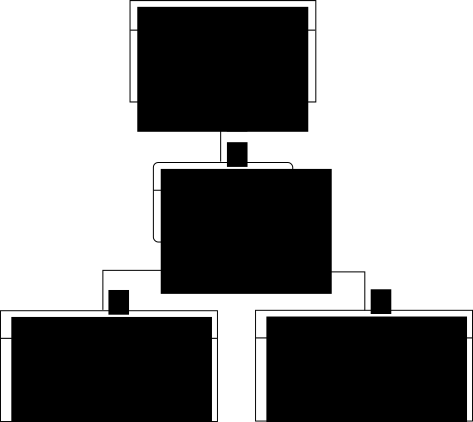
\includegraphics[scale=0.6,keepaspectratio=true]{./PeerAssetsDB.pdf}
 % PeerAssetsDB.pdf: 0x0 pixel, 300dpi, 0.00x0.00 cm, bb=
 \caption{Transaction relations}
 \label{fig:txn_relations}
\end{figure}

\subsection{Asset transaction}
Two types of asset transactions are defined.
The ``Card transfer transaction'' is a transaction to exchange an existing set of asset tokens.
The ``Card issue transaction'' is the special case where asset tokens are created, similar to Bitcoin's~\cite{Nak08} coinbase transaction.
Asset transactions can be linked to their deck spawning transaction by walking up the transaction chain until the deck spawning transaction is reached.
However, walking this chain is not trivial in either direction as transactions can have multiple in- and outputs which may not hold asset transactions.
Therefore tagging the transactions allows walking the chain with fewer transaction lookups.
The common denominator for all asset transactions is their deck spawning transaction.
Therefore it makes sense to tag asset transaction by the id of their deck spawning transaction.
The resulting transaction outputs for an asset transaction look as follows:

\begin{scriptsize}\begin{verbatim}
OP_RETURN <data>
OP_DUP OP_HASH160 <change_address_pk_hash> OP_EQUALVERIFY OP_CHECKSIG
OP_DUP OP_HASH160 <pk_hash_for_tag(deck_spawn_txid)> OP_EQUALVERIFY OP_CHECKSIG
\end{verbatim}\end{scriptsize}

Figure \ref{fig:txn_relations} illustrates the one-to-many relationship between the spawning and issuing transactions.
The procedure of generating the tag address from the create\_txn\_id is visualised through fnc\_tag\_address.
Note that the card issue transaction only differs from the transfer transaction by it's input being the create\_addr.


\subsection{Salting}
Note that only the deck spawning tag is salted. The id of the deck spawn transaction is a unique identifier and therefore doesn't require salting.
The deck spawning salt, or even the generated tagged address, can be hard coded in the client application making sure that all clients can easily query all ``deck spawning'' transactions.


\section{Conclusion}
Tagging transactions allows the creation of thin clients for blockchain applications that rely on historical data.
This is accomplished by using only standard lookup functions for addresses and transactions.
Tag address creation based on generating the private key from a publicly known seed results in insecure addresses.
However, tag addresses should not be used for value storage and therefore a secure address in not needed for this purpose.
An alternative could be to generate address' the public key based on the tag and salt.
This makes funds sent to it practically unspendable, and can act as a Proof-of-Burn mechanism to prevent ``tag spamming''.
Or a tag address can be generated from a secret tag while only communicating the tagged address itself, which would make the funds only spendable by the creator if a secure salt is chosen.
By not sending funds to an unspendable address, they can be redeemed by anyone knowing or guessing the tag and salt, leaving the blockchain some extra puzzles.


\begin{thebibliography}{9}

\bibitem{Nak08}
  S. Nakamoto,
  \emph{Bitcoin: A Peer-to-Peer Electronic Cash System},
  \url{https://bitcoin.org/bitcoin.pdf},
  2008.

\bibitem{King12}
  S. King, S. Nadal,
  \emph{PPCoin: Peer-to-Peer Crypto-Currency with Proof-of-Stake},
  \url{https://peercoin.net/whitepaper},
  2012.

\bibitem{Ros12}
  M. Rosenfeld,
  \emph{Overview of Colored Coins},
  \url{https://bitcoil.co.il/BitcoinX.pdf},
  2012.

\bibitem{Wui12}
  P. Wuille,
  \emph{Hierarchical Deterministic Wallets},
  \url{https://en.bitcoin.it/wiki/BIP_0032},
  2012.

\bibitem{Lee13}
  J. Lee,
  \emph{Peershares whitepaper},
  \url{https://wiki.peercointalk.org/index.php?title=Peershares_whitepaper},
  2013.

\bibitem{Emeth}
  Emeth,
  \emph{PeerMessage},
  \url{https://github.com/Peerapps/Peerapps/tree/master/peermessage}.

\bibitem{Pchem}
  Peerchemist,
  \emph{PeerAssets – Peercoin simple assets},
  \url{http://peerbox.me/psa/PSA.pdf},
  2016.

\bibitem{Matja}
  Matja,
  \emph{bitcoin-tool},
  \url{https://github.com/matja/bitcoin-tool}.

\bibitem{Blockr}
  \emph{Blockr},
  \url{http://blockr.io}.

\end{thebibliography}

\end{document}
